\documentclass[xcolor=dvipsnames,table]{beamer}

\usepackage{latexsym}
\usepackage[utf8]{inputenc}
\usepackage[brazil]{babel}
\usepackage{amssymb}
\usepackage{amsmath}
\usepackage{stmaryrd}
\usepackage{fancybox}
\usepackage{datetime}
\usepackage[T1]{fontenc}
\usepackage{graphicx}
\usepackage{graphics}
\usepackage{url}
\usepackage{algorithmic}
\usepackage{algorithm}
\usepackage{acronym}
\usepackage{array}

\newtheorem{definicao}{Definio}
\newcommand{\tab}{\hspace*{2em}}

\mode<presentation>
{
  \definecolor{colortexto}{RGB}{0,0,0}
 
  \setbeamertemplate{background canvas}[vertical shading][ bottom=white!10,top=white!10]
  \setbeamercolor{normal text}{fg=colortexto} 

  \usetheme{Warsaw}
}

\title{Apresentação da disciplina} 

\author{
  Esdras Lins Bispo Jr. \\ \url{bispojr@ufg.br}
  } 
 \institute{
  Física para Ciência da Computação \\Bacharelado em Ciência da Computação}
\date{\textbf{27 de setembro de 2016} }

\logo{\includegraphics[width=1cm]{images/ufgJataiLogo.png}}

\begin{document}

	\begin{frame}
		\titlepage
	\end{frame}

	\AtBeginSection{
		\begin{frame}{Sumário}%[allowframebreaks]{Sumário}
    		\tableofcontents[currentsection]
    		%\tableofcontents[currentsection, hideothersubsections]
		\end{frame}
	}

	\begin{frame}{Plano de Aula}
		\tableofcontents
		%\tableofcontents[hideallsubsections]
	\end{frame}
	
	\section{Sobre a Disciplina}
	\subsection{Professor}
	\begin{frame}{Professor}
		\begin{columns}
			\column{.4\textwidth}  		
		  		\begin{center}
		    		\includegraphics[height=.5\textheight]{images/esdras.png}
		  		\end{center}
			\column{.6 \textwidth}  		
				\begin{block}{Formação}
					\begin{center}
						{\normalsize {\bf Bacharel} em Sistemas de Informação\\
						{\bf Mestre} em Representação Conhecimento (IA)}
					\end{center}
				\end{block}		  		
		  		\begin{block}{Quem?}
		  			\begin{center}
						{\bf Esdras Lins Bispo Jr.} \\ Recife, Pernambuco.
					\end{center}
				\end{block}
		\end{columns}
	\end{frame}
	
	\subsection{Informações Importantes}
	\begin{frame}{Informações Importantes}
		\begin{block}{Professor}
			\begin{itemize}
				\item Esdras Lins Bispo Jr.
				\item \url{bispojr@ufg.br}
				\item Sala 18, 1º Andar (Bloco Novo dos Professores)
			\end{itemize}
		\end{block}
	\end{frame}	 
	
	\begin{frame}{Informações Importantes}
		\begin{block}{Disciplina}
			\begin{itemize}
				\item Física para Ciência Computação
				\item 17h20-19h00 (Terça, Sala 13, CA1)\\
					  17h20-19h00 (Quinta, Sala 13, CA1)
				\item Dúvidas: 19h00 - 20h00 (Quinta)\\
					  {\color{red}[é necessário confirmação comigo]}
				\item \url{www.facebook.com/groups/fcc.rej.2016.2}
			\end{itemize}
		\end{block}
	\end{frame}
	
	\begin{frame}{Informações Importantes}
		\begin{block}{Metodologia}
			\begin{itemize}
				\item Aulas expositivas;
				\item Testes;
				\item Prova;
				\item Exercícios-Bônus.
			\end{itemize}
		\end{block}
	\end{frame}
	
	\begin{frame}{Informações Importantes}
		\begin{block}{Testes}
			\begin{itemize}
				\item Teste 1 $\Rightarrow$ 20\% da pontuação total (11 de outubro);
				\item Teste 2 $\Rightarrow$ 20\% da pontuação total (08 de novembro);
				\item Teste 3 $\Rightarrow$ 20\% da pontuação total (29 de novembro);
				\item Teste 4 $\Rightarrow$  20\% da pontuação total (15 de dezembro).
			\end{itemize}
		\end{block}
		\begin{block}{Avaliação}
			\begin{itemize}
				\item Prova $\Rightarrow$  20\% da pontuação total \\
				(24 de janeiro e 02 de fevereiro).
			\end{itemize}
		\end{block}
		\begin{block}{Exercícios [Bônus]}
			\begin{itemize}
				\item Somatório dos exercícios.
			\end{itemize}
		\end{block}
	\end{frame}
    
    \begin{frame}{Informações Importantes}
		\begin{block}{Exercícios-Bônus}
			\begin{itemize}
				\item Semanalmente serão disponibilizados exercícios-bônus (EB) valendo 0,5 ponto na média (segunda-feira, normalmente); \pause
                \item Será dado um prazo para as candidaturas\\
                (normalmente um dia); \pause
                \item Será dada prioridade às candidaturas aos seguintes alunos: \pause
                	\begin{enumerate}
                    	\item Respondeu a nenhum EB; \pause
                        \item Respondeu a um EB; \pause
                        \item Respondeu a dois EBs; \pause
                        \item e assim por diante.
                    \end{enumerate} \pause
                \item Haverá sorteio entre candidatos dentro da mesma prioridade; \pause
            	\item Uma semana após, o candidato apresentará a sua resposta [texto escrito e slides] (normalmente na terça, 19h00).
			\end{itemize}
		\end{block}
	\end{frame}
	
	\begin{frame}{Informações Importantes}
		\begin{block}{Avaliação}
			O cálculo da média final será dada da seguinte forma:
			\begin{itemize}
				\item MF = MIN(10, PONT)
			\end{itemize}
			em que MIN representa o mínimo entre dois valores e PONT representa a pontuação total obtida em toda a disciplina.
		\end{block} \pause
		\begin{exampleblock}{Previsão de Término das Atividades}
			21 de fevereiro de 2017
		\end{exampleblock}
	\end{frame}
	
	\subsection{Distintivos Digitais}
	\begin{frame}{Distintivos Digitais}
		\begin{block}{Como será?}
			Os alunos que estiverem entre as 10 melhores notas de cada avaliação receberão um distintivo digital.
		\end{block} \pause
		\begin{block}{Quantos distintivos existem?}
			\begin{itemize}
				\item {\sc Top One}
				\item {\sc Top Five}
				\item {\sc Top Ten}
			\end{itemize}
		\end{block}
	\end{frame}
	
	\begin{frame}{Distintivos Digitais}
		\begin{block}{}
			\begin{center}
	    		\includegraphics[height=.65\textheight]{images/badges/top-ten.png}
	  		\end{center}		
	  		Obter a 6ª ou até a 10ª melhor nota da turma em uma avaliação. 
		\end{block}
	\end{frame}
	
	\begin{frame}{Distintivos Digitais}
		\begin{block}{}
			\begin{center}
	    		
\includegraphics[height=.65\textheight]{images/badges/top-five.png}
	  		\end{center}		
	  		Obter a 2ª ou até a 5ª melhor nota da turma em uma avaliação. 
		\end{block}
	\end{frame}
	
	\begin{frame}{Distintivos Digitais}
		\begin{block}{}
			\begin{center}
	    		
\includegraphics[height=.65\textheight]{images/badges/top-one.png}
	  		\end{center}		
	  		Obter a melhor nota da turma em uma avaliação. 
		\end{block}
	\end{frame}
	
	\begin{frame}{Distintivos Digitais}
		\begin{block}{Pontuação}
			\begin{itemize}
				\item Obter um {\sc Top One}: 12 pontos;
				\item Obter um {\sc Top Five}: 6 pontos;
				\item Obter um {\sc Top Ten}: 3 pontos.
			\end{itemize}
		\end{block} \pause
		\begin{exampleblock}{No final da disciplina...}
			Os três primeiros que obter maior pontuação ganharão prêmios.
		\end{exampleblock} \pause
		\begin{block}{Por que estamos usando distintivos digitais?}
			\begin{itemize}
				\item Pode aumentar a motivação dos alunos; \\ \pause
				{\color{blue} (Estou pesquisando para saber se isto é verdade...)}
			\end{itemize}
		\end{block}
	\end{frame}

	\begin{frame}{Informações Importantes}
		\begin{block}{Conteúdo do Curso}
			\begin{enumerate}
				\item Fundamentos Matemáticos;
				\item Medidas Físicas e Vetores;
				\item Movimentos;
				\item Trabalho e Energia;
				\item Colisões;
				\item Hidrostática;
				\item Outros tópicos.
			\end{enumerate}
		\end{block}
	\end{frame}

%------------------------------------------
	\section{Pensamento}
	\begin{frame}{Pensamento}
  		\begin{center}
    		\includegraphics[width=7cm]{images/pensamento.png}
  		\end{center}
	\end{frame}
	
	\begin{frame}{Pensamento}
		\begin{columns}
			\column{.4\textwidth}  		
		  		\begin{center}
		    		\includegraphics[height=.6\textheight]{images/einstein.jpg}
		  		\end{center}
			\column{.6\textwidth}  		
				\begin{block}{Frase}
					\begin{center}
						{\large Minhas ideias levaram as pessoas a reexaminar a física de Newton. Naturalmente, alguém um dia irá reexaminar minhas próprias ideias. Se isto não acontecer, haverá uma falha grosseira em algum lugar.}
					\end{center}
				\end{block}		  		
		  		\begin{block}{Quem?}
		  			\begin{center}
						{\bf Albert Einstein (1879-1955)} \\ Físico alemão.
					\end{center}
				\end{block}
		\end{columns}
	\end{frame}
%------------------------------------------
	\section{Introdução}
	
	\subsection{Qual a relevância da Física para Computação?}
	\begin{frame}{Relevância da Física para Computação}
		\begin{block}{Criar efeitos de animação realísticos}
			\begin{center}
	    		\includegraphics[height=.7\textheight]{images/rotacao-cubo.png}
	  		\end{center}
		\end{block}
	\end{frame}
	
	\begin{frame}{Relevância da Física para Computação}
		\begin{block}{Criar jogos realísticos}
			\begin{center}
	    		\includegraphics[height=.7\textheight]{images/slingshot.png}
	  		\end{center}
		\end{block}
	\end{frame}
	
	\begin{frame}{Relevância da Física para Computação}
		\begin{block}{Construir simulações e modelos}
			\begin{center}
	    		\includegraphics[height=.7\textheight]{images/boeing737.jpg}
	    		\\Simulador do Boeing 737
	  		\end{center}
		\end{block}
	\end{frame}
	
	\begin{frame}{Relevância da Física para Computação}
		\begin{block}{Gerar arte a partir de código}
			\begin{center}
	    		\includegraphics[height=.7\textheight]{images/fractais.jpg}
	    		\\Fractais encontrados na natureza
	  		\end{center}
		\end{block}
	\end{frame}
	
	\subsection{O que é Física?}
	\begin{frame}{O que é Física?}
		\begin{block}{Definição Rasteira}
			A Física é o estudo das leis naturais que governam como as coisas se comportam. Estas coisas se referem ao espaço, tempo e matéria.
		\end{block} \pause
		\begin{block}{Aspectos importantes}
			\begin{itemize}
				\item Formular leis gerais que governam: \pause
					\begin{itemize} 
						\item o comportamento da matéria;
						\item o movimento da matéria no tempo e no espaço;
					\end{itemize} \pause
				\item Predizer como a matéria se move e interage, seus componentes, uns com os outros: \pause
					\begin{itemize}
						\item previsão de eclipses (leis da gravidade);
						\item voo de aviões (aerodinâmica).
					\end{itemize}
			\end{itemize}
		\end{block}	
	\end{frame}
	
	\begin{frame}{O que é Física?}
		\begin{block}{Mecânica}
			 Mecânica é o ramo da física que estuda as leis que governam o movimento dos objetos e como estes movimentos influenciam o ambiente.
		\end{block} \pause
		\begin{block}{Outros aspectos importantes}
			\begin{itemize}
				\item Muitas coisas se comportam de acordo com as leis da Física; \pause
				\item Estas leis podem ser descritas por equações matemáticas; \pause
				\item É possível fazer uma previsão de movimentos.
			\end{itemize}
		\end{block}	
	\end{frame}
	
	\subsection{Programação e Física}
	\begin{frame}{Programação e Física}
		\begin{figure}		
			\begin{center}
	    		\includegraphics[height=.5\textheight]{images/fluxograma.png}
	    		\caption{Passos para a programação em Física}
	  		\end{center}
	  	\end{figure}
	\end{frame}
	
	\begin{frame}{Exemplo}
		\begin{block}{Bola quicando}
			\begin{center}
	    		\includegraphics[height=.7\textheight]{images/bola-quicando.png}
	    		\\Exemplo de bola quicando com HTML5 e JavaScript
	  		\end{center}
		\end{block}
	\end{frame}
	
	\begin{frame}{Bônus (0,5 pt)}
		\begin{block}{Desafio}
			{\bf Q 1.67} Um núcleo de ferro tem um raio de $5,4 \times 10^{-15}$m e uma massa de $9,3 \times 10^{-26}$ kg.
			\begin{enumerate}
				\item Qual é sua massa por unidade de volume, em kg/m$^3$?
				\item Se a Terra tivesse a mesma massa por unidade de volume, qual seria o seu raio?
			\end{enumerate}
			(A massa da Terra é $5,98 \times 10^{24}$kg.) 
		\end{block} \pause
		\begin{block}{Informações úteis}
			\begin{itemize}
                \item Candidaturas até quinta (29 de setembro, 17h20);
                \item Apresentação e resposta por escrito $\rightarrow$ \\Terça (04 de outubro, 19h00);
                \item 20 minutos de apresentação.
			\end{itemize}
		\end{block} 
	\end{frame}
	
	\begin{frame}
		\titlepage
	\end{frame}
	
\end{document}